\documentclass{article}
\usepackage{graphicx}
\usepackage{xcolor}
\usepackage[margin=3cm]{geometry} % margins might need to change in the future check with professor adam 
\setlength{\parindent}{0pt}
\usepackage{pgfgantt}

\usepackage{times}
\usepackage{fancyhdr,graphicx,amsmath,amssymb}
\usepackage[ruled,vlined]{algorithm2e}
\include{pythonlisting}


\begin{document}

\begin{center}
    \Large \textcolor{red}{\textbf{Electronics and Computer Science} \\[0.1cm]} 

    \large \textcolor{red}{Faculty of Engineering and Physical Sciences \\[0.1cm]} 

    \textcolor{red}{University of Southampton \\[1cm]} 

    \vspace{1cm} 

    \textcolor{red}{\textbf{\large Ashwinkrishna Azhagesh} \\[0.5cm]}

    \textbf{25/03/2025} \\[1cm] 

    \textbf{\large An AI Approach to Chaotic Physical Systems: } \\[1cm]

    \vspace{0.5cm}

    Project supervisor: \textbf{Adam Peugeot} \\[0.3cm] 
    Second examiner: \textbf{David Millard} \\[1cm]

    Progress report submitted for the award of \\[0.1cm]

    \textbf{\large Bachelors of Science} 
\end{center}

\newpage

{\Huge \textbf{Abstract}}\\[1cm]

Empirical laws are mathematical generalisations found through observing the physical world. It has taken us centuries of gathering data, keen research along with repeated experiments, and no doubt plenty of talented scientists to discover these laws. Leading us to understand everything from the mysteries that govern the collision of two objects to the shape of the path planets thread upon.\\

Recent advances in neural networks including increases in computational power permit us to train models, that replicate, fasten and automate our discovery of empirical laws. This extends to even noisy chaotic systems such as the double pendulum. Combined with white box models, symbolic regression and explanable A.I., we can peer into the "mind," of how such models, process data and conclude their observations. Human congition is inherently finite in its capacity for thought and observational ability, has been historically overcome through the development of new tools such as the microscope. Similarly, congitive biases can be mitigated, by utillising artificial intelligence, which is a rapidly emerging technology capable of expanding our perception and analysis.\\       


\newpage

\fbox{\underline{\textbf{Statement of Originality}}}
\\[0.5cm]

- I have read and understood the ECS Academic Integrity information and the University’s
Academic Integrity Guidance for Students.\\

- I am aware that failure to act in accordance with the Regulations Governing Academic Integrity
may lead to the imposition of penalties which, for the most serious cases, may include
termination of programme.\\

- I consent to the University copying and distributing any or all of my work in any form and
using third parties (who may be based outside the EU/EEA) to verify whether my work
contains plagiarised material, and for quality assurance purposes.\\

\fbox{
\underline{\textbf{You must change the statements in the boxes if you do not agree with them.}\\
}}
\\[0.5cm]

We expect you to acknowledge all sources of information (e.g. ideas, algorithms, data) using
citations. You must also put quotation marks around any sections of text that you have copied
without paraphrasing. If any figures or tables have been taken or modified from another source,
you must explain this in the caption and cite the original source.\\

\fbox{
\underline{\textbf{I have acknowledged all sources, and identified any content taken from elsewhere.}\\
}}
\\[0.5cm]

If you have used any code (e.g. open-source code), reference designs, or similar resources that
have been produced by anyone else, you must list them in the box below. In the report, you must
explain what was used and how it relates to the work you have done.\\


\fbox{
\underline{\textbf{I have not used any resources produced by anyone else.}\\
}}
\\[0.5cm]

You can consult with module teaching staff/demonstrators, but you should not show anyone else
your work (this includes uploading your work to publicly-accessible repositories e.g. Github, unless
expressly permitted by the module leader), or help them to do theirs. For individual assignments,
we expect you to work on your own. For group assignments, we expect that you work only with
your allocated group. You must get permission in writing from the module teaching staff before
you seek outside assistance, e.g. a proofreading service, and declare it here.\\

\fbox{
\underline{\textbf{I did all the work myself, or with my allocated group, and have not helped anyone else.}\\
} }
\\[0.5cm]

We expect that you have not fabricated, modified or distorted any data, evidence, references,
experimental results, or other material used or presented in the report. You must clearly describe
your experiments and how the results were obtained, and include all data, source code and/or
designs (either in the report, or submitted as a separate file) so that your results could be
reproduced.\\

\fbox{
\underline{\textbf{The material in the report is genuine, and I have included all my data/code/designs.}\\
}}
\\[0.5cm]

We expect that you have not previously submitted any part of this work for another assessment.
You must get permission in writing from the module teaching staff before re-using any of your
previously submitted work for this assessment.\\

\fbox{
\underline{\textbf{I have not submitted any part of this work for another assessment.}\\
}}
\\[0.5cm]

If your work involved research/studies (including surveys) on human participants, their cells or
data, or on animals, you must have been granted ethical approval before the work was carried
out, and any experiments must have followed these requirements. You must give details of this in
the report, and list the ethical approval reference number(s) in the box below.\\

\fbox{
\underline{\textbf{My work did not involve human participants, their cells or data, or animals.}\\
}}
\\[0.5cm]


ECS Statement of Originality Template, updated August 2018, Alex Weddell aiofficer@ecs.soton.ac.uk\\


\newpage 

{\Huge \textbf{Abstract}}\\[1cm]


I would like to thank my supervisors, Professor Adam Peugeot and Professor David Millard, for all the help and advise I received throughout this project. \\


\newpage

\tableofcontents 

\newpage
\addcontentsline{toc}{section}{Abstract}
\addcontentsline{toc}{section}{Statement of Originality}



\section{Introduction: }

\subsection{Motivation: }

As there is more data being generated than ever before and new experiments, we need a systematic and au-
tomatic way to deduce various mathematical patterns and laws in these data. Through the use of symbolic
regression we can utilise these data, and in an explainable manner deduce various new physical laws. In this
research I have also extended this beyond physics and have applied this to biological data sets which is a novel
application of this method. Perhaps extend this beyond or add a sectionsaying this can also be applied to nlp
and that it can learn the rules in language and writing etc.
Talk a little about the way this is used outside of this niche use case, and in research, so of course I need to look
and research into this.\\

\section{Previos Work: }

\subsection{Literature Review: }

\subsection{ Introduction: }
  
Humanity has spent millennia observing the world, creating concepts that describe the variables, such as mass and force, to derive laws. In physics, like with
all human endeavours, new discoveries and ways of thought are based upon previous works, creating
a natural bias in the way new problems are approached. All existing theories, are therefore
somewhat biased, this combined with our pre-existing bias in our biological brains, can introduce some
hurdles to our future progress \cite{Wood2022} \cite{Schmidt2009}.\\

In the 17th Century, Kepler had gotten his hands on the word’s most precise data tables on the orbits
on planets, using this he spent close to half a decade, and after numerous unsuccessful
attempts, he had began a scientific revolution at the time, describing Mar’s orbit to be an ellipse \cite{kepler}.
In essence, scientists throughout history, much like Kepler, have spent a great deal of time, discovering
the right expressions to match the relevant data they have, this at it’s core is symbolic regression. Now,
a few centuries later, even with exponential increases in orders of magnitude in our capability to perform
calculations through computers, the process of discovering natural laws and the way to express them,
has to some extent resisted automation.\\


One of the core challenges of physics and artificial intelligence, is finding analytical relations automatically, discovering a symbolic expression that accurately matches the data from an unknown function.
This problem, due to it’s nature, is NP-hard \cite{Hope2023} in principle. The vastness of the space
of mathematical constants, adds to the difficulty. 
This literatire review aims to present the recent advances in discovery of emphirical laws through data powered by artificial intelligence. It focuses on methodoogies that dimish human bias through seeking solutions without assumptions. We will explore various techniques employed to achieve these goals, which includes reducing the search space, and analyse the effectivness of these methods.\\  

\begin{figure}[h] 
    \centering
    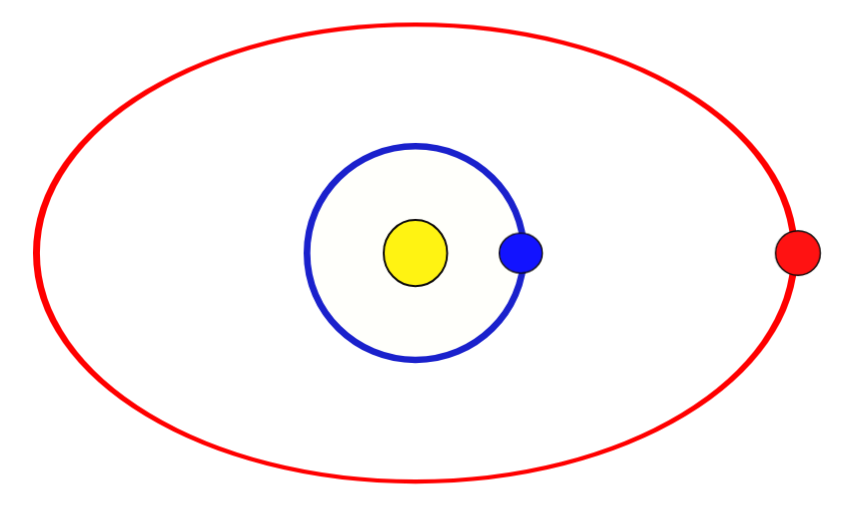
\includegraphics[width=7cm]{Sun_Mars_Orbit} 
    \caption{This is the orbit of Earth and Mars around the Sun.}
    \label{fig:Orbit} 
\end{figure}


\subsection{Symbolic Regression: }

Symbolic regression, is a technique that analyses and searches over the space of traceable mathematical
expressions to find the best fit for a data set. By not requiring prior information about the model,
it is unbiased. There are a plethora of various strategies that have been implemented in solving for
empirical laws \cite{Schmidt22009}, we will explore some of them below. It is also worth mentioning, that unlike other
well-known techniques for regression, (eg: neural networks), that are essentially black boxes, symbolic
regression, aims to extract white-box models and is easy to analyse.\\

\begin{center} 
  \textbf {\Large  Brute Force:}
\end{center}
Symbolic Regression (SR), is interpretable \cite{Aldeia2022}, unlike Neural Networks (NN), which are often considered more explainable. The difference is interpretability allows us to comprehend how the model works,
like observing how gears move in a glass box, while explainable means you get an overview of why a
certain output was achieved, even without knowing the full nuances of it’s inner workings.\\

There however, are some challenges associated with SR, in comparison to function fitting (NN). SR,
starts with nothing, a blank slate, and it has to learn the entire expression \cite{Cranmer2020}, unlike function fitting
which just tweaks an already existing function. The exponential search space \cite{Worm2014} , causes it to be
extremely computationally expensive to explore all possibilities. This combined with the face that,
most optimisation algorithms expect a smooth search space \cite{Makke2024}, however SR lack’s smooth interpolation, small changes in the potential solutions (expression), ie: $ x3 and x3 + 0.1$ can significantly alter
the the output. Finally, if the nature of the problem is badly posed \cite{Rivero2022}, there might potentially be
multiple solutions to the same data. Imagine trying to find a single polynomial equation with only two
points of data, the need to balance finding accurate expressions with finding the most simplistic and
generalisable fit, is sometimes troublesome.\\

The brute force approach of simply trying all possible combinations of symbolic expressions within some defined space. The model will subsequently increase the complexity over time, and will stop when either the fitting errors lowers below some defined limit or exceeds the upper limit of runtime. While in theory can solve all of our problems, in practise takes longer than the age of our universe to finish. In essence it's like searching for a singular drop in the ocean. Thankfully, there are some ways of pruning the search space, and drastically reducing the time taken to solve for the most accurate expression. \\ 

\begin{center} 
  \textbf {\Large Partial Derivatives:}
\end{center}

Partial derivatives, of some function f, with multiple variables such as x and y, is it's dervative with respect to one of those two variables, while the other variables in the function are kept constant. Formally, given a function with two or more variables, $f(x_1, x_2, \ldots, x_n) $, the partial derivative of $f$ with respect to $x_i$, where $x_i$ is some value $x$ in $(x_1, x_2, \ldots, x_i, \ldots, x_n)$, gives the rate of change of $f$ with respect to $x_i$. It is calculated by taking the ith derivative of $f$ with respect to $x_i$, whilst holding the other variables fixed. \cite{Stewart2012} \cite{Smith2012} \\

The partial derivative of a function $f(x,y)$ with respect to $x$ is denoted $\frac{\partial f}{\partial x}$ \cite{Kelly2021} and is defined: \\ 

\begin{center}

  $\frac{\partial f}{\partial x} = \lim_{h \to 0} \left[ \frac{f(x+h, y) - f(x,y)}{h} \right]$
\end{center}


Once you pass in the experimental data, you can pre-process the data, using calculated partial derivatives, for every pair of existing variables. Many physical laws, involve rates of change, and partial
derivatives help us represent them. Furthermore it also guides the search process, as the algorithm can
use the derivative to accurately represent the underlying laws involved. Through comparing how well
the partial derivatives derived through the experimental data compared to the potential expression,
the algorithm can assess the accuracy and feasibility of the expressions involved. This strategy can
even be extended to prune the search space further, this could be achieved through incorporating
knowledge of physics into the constraints for the partial derivatives. These concepts will be illustrated
with an example below.\\


Consider a iron rod, that has been heated up, such that it is hotter on one side than the other. Now it is intuitive to say that closer to the heat source, the temperature will be higher than further along the rod, where it will be colder. We can illustrate this temperature distribution with a function:  \\

\begin{center}
$T(x,y,z)$
\end{center}

where T is the temperature at a point in the rod, and (x,y,z) are the coordinates along the axis in 3 dimensions. This leads to these 3 partial derivatives: \\ 

\begin{center}
 $\frac{\partial T}{\partial x}, \  \frac{\partial T}{\partial y}, \  \frac{\partial T}{\partial z}$
\end{center}

These partial derivatives, gives us information about the direction and magnitude of heat flow at various points on the rod. The algorithm then searches for an equation T(x,y,z), that sufficiently predicts the observed temperature distribution and it's partial derivatives, deriving laws such as the heat transfer equations, or elasticity relationships.\\ 

\begin{center}
$\frac{\partial T}{\partial t} = \alpha \nabla^2 T$
\end{center}



Through using partial derivatives, we have in essence redefined the search criteria for the algorithm, through it's measure of the accuracy in comparison of potential solutions over the invariants represented in the experimental data \cite{Kelly2021} . This also leads to the pleasant finding, that it can additionally capture relationships that represent other identities of the system, beyond invariants and heat transfer equations. \\ 

You can subtly guide the type of laws that such an algorithm finds, by selectively picking the variables to input into the algorithm,. For example providing velocities and force to find laws of motion. \\ 





\begin{center} 
  \textbf {\Large Dimensional Analysis:}
\end{center}

Dimensional Analysis is a method of solving problems usually in maths and physics, where we analyse
the relationships between different physical quantities, by comparing their ”units.” It is a powerful
method of reducing the complexity of systems, enabling engineers and scientists to analyse problems
that we can’t even pose, much less solve the equations of \cite{Longo2021}.\\

Using the fact that numerous questions in science can be simplified by requiring the dimensions/units
of the right and left hand side of the expression to be equal, we can transform the question into
a smaller number of variables, which all have no dimension \cite{Blasiak2012}. It has been automated to find the integer powers of expressions and has proven to be useful especially when the power is an irrational number.\\

Here is a general strategy that showcases how dimensional analysis can be used:\\

Let's say we have a variable in an equation that can be broken down into it's fundamental units, such as (second, kilograms, ampere ...) to various powers. We can then take this, and represent each of the units as vectors, such that each of the fundamental units, is assigned a dimension, and it's important to note, this then allows us to represent any physical quantity as a product of these units, so let us construct a vector $v$, with $3$ integers, where each corresponding integer represents the power of each of the fundamental units.\\ 

Given that we want to derive an expression, such as $y = f(x_1, \dots, x_n)$  we can then create some matrix $M$. Each of the columns of the given matrix, is the unit vector $v$ of the corresponding variable $x_i$. We then need to define another vector to represent the units of y, which will be called $z$. If we let the solution be some vector $s$, solving $Ms = z$, this then lets us raise the powers on both sides, to elevate the independent variables, to make this equation dimensionally consistent.\\ 

Taking the null space of the matrix $M$, where $MV = 0$, allows us a basis to create a dimensionless group, allows for a simplification of the problem.\\

This is also more intuitive to understand physical phenomena, the nature of physics comprehension, making this vital in further understanding derived laws, making the process easier to explain and understand \cite{Taber2009}. Therefore, this is a crucial tool, for cultivating a deeper understanding of physics effectively \cite{Tenachi2023}. \\






\begin{center} 
  \textbf {\Large Genetic Programming:}
\end{center}


Genetic programming (GP), is a special evolutionary algorithmic technique, where the individuals are seen as programs that evolve, starting for a population, is iteratively "evolved," transforming the populations of individual programs, intro other populations. This new generation of programs are created using some genetic operations or survival criteria, mimicking natural evolutionary condition on earth.\\ 

A very basic overview, shows that genetic programming algorithms, consists of initializing the population, then evaluation of the said population through some predefined metrics and functions, followed by selection of the fittest programs based on the score given by the metric, and "genetic operation," such as reproduction, mutation and cross-over. The algorithm then iterates these steps thousands of times, through many generations, and finally terminates once the desired result has been achieved.\\

We can use genetic programming, and tweak the algorithm, and combine it with symbolic regression, to help us derive laws. \\

Consider modelling the various potential formulas as a tree, which is composed of various functions in the nodes. These functions can vary from arithmetic operations  , mathematical functions, or defined unique operators. Then we can program the fitness function \cite{Angeline1994}, and use it to measure how well the given potential expression in the population compares with the given databases, and given the nature of genetic programming, the better performing functions are more likely to be passed down into the next generation. Then after many iterations, we can give the solution with the best performance. \\ 

There are various ways to implement the fitness function, and for example we can use a criteria like this, along with mean squared error \cite{Liddle2009}:\\

\begin{center}
  $V = 2X + N \cdot ln(M/N) $
\end{center}

Here M is the mean squared error, and N is the number of data points, X is the number of parameters used on the genetic programming algorithm. The lower the value of V is, the better the model performs. The performance of this stratergy can then be evaluated with various other metrics, to judge how well the algorithm performs. \\ 




\section{PySR}

This section describes the relevent implementations that are completed as of 10 December 2024.\\ 

\subsection{Momentum Laws: }

To generate the dataset, I chose 100 data points, and created two variables mass (M) and acceleration (a), each represented in two dimensions. Then the data points were generated using $numpy.random.randn$ function. The force (F), was then calculated to be the produce of these two data sets. Mass and acceleration were concatenated along the same axis using $numpy.concatenate$, resulting in a combined dataset. This is partially because the model used here, $PySRRegressor$ expects a single array as input, and this helps highlight the relationship between these variables to the symbolic regression algorithm.\\ 

Then model performed symbolic regression, configured with 40 iterations along with a customer loss function, taken to be the squred diffrence between the prediction and the target variable. \\ 

\begin{center}
  
  $$
  {\boldsymbol{\mathcal{L}(\hat{x}, x) = (\hat{x} - x)^2}}
$$

\end{center}


The model was trained on this dataset, upon termination, it produced a list of potential candidate formulae, from which I manually identified the correct expression, $F = m \dot a$. \\



\begin{algorithm}[H]
\SetAlgoLined
\KwResult{A symbolic representation approximating \( F = M \cdot A \)}
\textbf{Initialization:} \\
Generate random data for mass (\( M \)) and acceleration (\( A \))\;
Compute target force values: \( F = M \cdot A \)\;
Combine \( M \) and \( A \) into input matrix \( X \)\;

\While{Symbolic regression process}{
  Train the symbolic regression model with the following settings:\;
  \textbf{Binary operators:} Multiplication (\(*\))\;
  \textbf{Unary operators:} None\;
  \textbf{Loss function:} Mean squared error between predictions and targets\;
  \textbf{Iterations:} 40\;

  \eIf{Current symbolic representation improves loss}{
   Update the symbolic model\;
   Save the current best expression\;
   }{
   Continue exploration of new symbolic expressions\;
  }
 }
\caption{Symbolic Regression for \( F = M \cdot A \)}
\end{algorithm}

\\
\\

Similarly, the other laws of momentum, were also dervied using this approach. \\ 
\\

\begin{align} \label{eq:impulse_momentum}
\mathbf{F} \Delta t &= \Delta \mathbf{p} = m(\mathbf{v}_f - \mathbf{v}_i) \\
m_1 \mathbf{v}_{1,i} + m_2 \mathbf{v}_{2,i} &= m_1 \mathbf{v}_{1,f} + m_2 \mathbf{v}_{2,f}
\end{align} 
%\subsection{Optimising the Symbolic Regression Algorithm: }

%\subsection{Neural Networks: }

%\subsection{ White Box models: }

\subsection{Pendulum Laws:}

The data is generated using numpy. The simulation involves, Euler's method to solve the pendulum's equation of motion. Through taking small and discrete steps, the method approximates the solution. The equation for a simple pendulum is given by: \\

\begin{center}
\begin{equation}
\alpha = -\frac{g}{L} \sin(\theta)
\end{equation}
\end{center}

\begin{description}
    \item[\(\alpha\)] angular acceleration (\(\text{rad/s}^2\))
    \item[\(g\)] acceleration due to gravity (\(\text{m/s}^2\))
    \item[\(L\)] length of the pendulum (\(\text{m}\))
    \item[\(\theta\)] angular displacement (\(\text{rad}\))
\end{description}

The Euler technique approximates the changes in angular velocity and displacement over some small step in time, as follows:\\

\begin{center}
\begin{align} 
\omega_{i+1} &= \omega_i + \alpha_i \Delta t \\
\theta_{i+1} &= \theta_i + \omega_{i+1} \Delta t 
\end{align}
\end{center}


The function iterates through a few hundred time steps, updating the angular velocity and displacement at each time step. To prevent errors accumulating due to numerical drift, which are small errors that accumulate and become significant due to the inherent nature of approximation methods like Eulers. To keep the values coherent, a wrap around operation is used to ensure the angular displacement is within the range of [\pi, -\pi] radians.\\ 

\subsection{Noise: }

In this section, I aimed to explore how noise affects the model, and potential ways to mitigate it. Continuing
onwards from the previous model, in the data generation step, noise was artificially added, and the results were
observed.\\

So in order to model the noise, I used the python random library, and generated random numbers between 0 and
an ever increasing amount of randomness, in oder to guage the accuracy as noise increased for the model. I was
also part\\

\subsubsection{How noise affects the model: }
So in order to add noise to the generated data set, I imported in random, and used the randn.int function. In order
to vary the inputs, another function was created that incrememntally passes in higher numbers as parameters
to the random function, allowing each set of generated data to incrememntally become more and more noisy.
Then the symbolic regression model is run on these new data sets, and the resulting equations levels of noise
are then plotted in a graph. Furthermore using the Time library to measure the amount of time it takes to run
the model as the amount of random error increases.
\subsubsection{How to mitigate noise in data: }
 Ways to mitigate the noise and it’s affects on the model were explored. Functions such as ”denoise,” in the
symbolic regression library helped to some extent. However after a certain point, such methods do not seem to
offer much assistance.\\
I also made my own denoise algorithm. I implemented various different denoise algorithms to see what effects
they had. Firstly I implemented a simple moving avergae as a way to mitigate the noise in the dataset. reword
this -¿ ” Simple and fast, smooths data well by averaging neighbors. However, it blurs sharp changes and is
sensitive to extreme outlier values, pulling the average significantly and distorting the signal.”
These were my results, this is the pseudo code, explain the alogrithm\\

The second denoise algoirthm I implemented is a median filter, and this is what effects it has, and this is how
i implemented it. Insert Pseudo code. reword: ”Excellent at removing spikes and preserving edges better than
averaging. Less affected by outliers. Can sometimes slightly distort the overall shape of the signal, especially
with large window sizes.”\\

Finally this is the third algorithm that I had implemented for denoising. Wavelet Denoising, this is the effects,
and this is the pesudo code. Reword this -¿ ”Transforms data to isolate noise, preserving both smooth and sharp
signal features effectively. More complex to understand and requires careful selection of wavelet type and pa-
rameters for optimal results, which can be tricky.”\\

\subsubsection{Modelling the noise: }

\section{Symbolic Regression from Scratch: }
\subsection{The core: }
The core and essential part of any symbolic regression model, lies in the way it at the simplest level, generates
and traverses the search tree of possible equations and expressions that may fit the data presented to it.
In order to save time, and to test if my expression generation was working as intended, i have started with sim-
ple 2 variable equaitons, and also pass in the speific operations used in the equation. Furthermore this is also
extended to handle constants and more later on.
enter in the pseudo code here.\\

Then I further improved this, by designing a resursive way to generate these expressions, to allow to generate
more robust equations from the given variables. Also this is dynamic, so it can
enter in pseudo code.\\

\subsubsection{ Exploiting Physical Properties: }

The next step is to then start to truncate these generated expressions as much as possible to prune the search
tree. One of the ways you can do this is through exploiting the symmertrical property of physical equations and
how they are mathematically equivalent. Such as removing duplicate expressions.\\
This is how I achieved that.\\
Give pseudo code here.\\

\subsubsection{Dealing with constants:}

Another way i further pruned the amount of expression, is through filtering all the expressions generated through
the newer recursive generator, by removing all the expressions that did not contain all the specified variables.
This is in order to save further time later on during the evaluation seciton.
Insert in pseudo code:

\subsubsection{Dealing with powers:}
So appling powers to expressions, I applied the power to the expression. This also allows you to prune the
search tree further by not needed to generate redundant expressions with powers.
This is the pseudo code.
Then I filtered based on if the expression contained the power, this allows me to further prune the tree. In a more
robust model, this is dervied from scratch, however for the sake of computation time, and flexibility, I decided
to proceed with this approach as it saves some time.
this is the pseudo code.
\subsubsection{Chaining powers and constants:}
The next step is to chain together powers and constants, such that both are applied to the expressions. It can
already be chained as with the design it already has. However it needs to be filtered poperly in order to maintain
the least amount of expressions possible.
Te constants filter can be used, but the powers are inside the constants, and therefore the older power filter does
not work as intended. Therefore i needed to redesign it such that it will function recursively.
This is the code.
However, sometimes this gives off constants that are chained, such as sin(sin()), and so to filter this futher, I
want to filter out expressions with more than one instant of the constant that is chained.
this is the code - filter single constant
\subsubsection{Loading data:}

Next I needed a way to load the data I has typed up. At this point I was focused on testing as quick as possible
and in order to proceed in a prompt manner I made up some dummy data values. Afterwards I made the decision
to keep the data as a numpy array, because this will be faster then a text file, there are some various reasons for
this, such as numpy arrays being stored in memory, the efficiency of the nderlying data format it is stored in
(binary), and finally numpy uses c, and so it vectorises operations, making it far faster.
Insert in pseudo code.


As you can see I check if the number of variables entered matches the shape of the arrary in X, which here is the
input data, and y being the target data, as in the final result. Ie x contains the mass and acceleration values, and
y is the array of the result of the equation f = ma, so it only contains the value of f in it. This is a basic check to
make sure the number of columns all have a corresponding variable.

\subsubsection{Evaluating expressions:}
Next I evaluate the expressions that I had generated, and i assign the variables to a column of the data, in in-
creasing order. Then this is substituted into the equation, and the expressions are run, and there is an array
of outputs of the expression. This essentially evaluates every generated expressions that has been pruned, and
returns a np arrya of the results of those expressions based on the input data.
insert in pseudo code here.
Then like the paper suggested, insert in paper here, I used a medium error description length loss function, and
have implemented it in the same way as in the paper. Using error squared, making all the errors positive, and
added 1 as a constant to ensure that all the errors are greater than the value, when taking the log.
Insert in pseudo code.
Then furthermore I also implemented 2 other loss algorithms, specifically root mean squared loss as well as
mean absolute error.
insert in pseudo code.
This was to help bridge and improve upon the loss algorithm used in the paper, as these two have their own
advantages, and a combined hybrid approach seemed smarter.
Explain why later.
\subsection{Polynomial Fit Module: }
Now that the simple, core of the algorithm works, and is adapted to take care of contants, powers, variables,
generate expressions, and filter out the redundancy using physical properties of the world such as symmtery,
I now aimed to futher extend the program by writing a polynomial fit module. The aim of the polynomial fit
technique is to.
Why: Many functions in physics (or parts of them) are low-order polynomials.
Why: It’s a computationally very cheap method for this specific function class.
How: It attempts to fit the given data to a sum of polynomial terms.
How: It generates all possible polynomial terms up to a specified low degree (e.g., degree 4).
How: For each data point, this creates a linear equation where the unknowns are the polynomial coefficients.
How: It solves the resulting system of linear equations using standard methods like least squares.
How: The Root Mean Squared Error (RMSE) of the fit is calculated.

How: If the RMSE is below a predefined tolerance (p ol), thepolynomialisacceptedasasolution.
Effect: It acts as a fast base case in the recursive algorithm, quickly solving problems that are simple polynomi-
als.
Effect: It can also solve sub-problems that are transformed into polynomials by other modules (e.g., dimen-
sional analysis, inverting the function).

\subsubsection{Data Loading:}
So to start, I began by creating the data loading function. The aim was to take in a numpy array, with the data,
along with a list of variables. Then comparing the shape of the data column and the number of variables in order
to make sure the input is sufficient.
This is the pseudo code. 


\subsubsection{Generating polynomial expressions:}

Then the next step is to generate polynomaial expressions, and then it will return a list of polynomial expres-
sions on the list.
Pseudo conclude


\subsubsection{Filtering the Polynomial expressions:}


The filtere xpressionsf unctionprogrammaticallyf ilterssymbolicexpressionsusingstructuralandsemanticconstraints.Lev
suitedf orlarge − scalesymbolicf ilteringtaskswherestrictmathematicalstructuremustbeenf orced.
insert in pseudo code.
This initial version only worked for symblic constants, ie sin, cos etc, and didn’t work for numbers, or nteger
coefficients, i caught this error during testing and I rewrote the function so that it works for integer coefficients


\subsubsection{Evaluating expressions:}

Now I need to take the filtered expressions, and try fit the model to the dataset np array. The model fitting
logic function fits polynomial expressions to input data by finding the best set of coefficients that minimize the
error between the predicted and actual output values. It tests multiple polynomial degrees (up to a specified
maximum) and selects the one that provides the lowest error, ensuring an optimal balance between accuracy
and complexity.
I use root mean squared error to calculate the loss, and the funciton returns a list of loss, per expression. 

So i take an expression, then I substitute in the variables using the input data, calculate the predicted y value of
the said equation, then take it away from the true value of y the target and then use that to calculate the rmse.
pseudo code.
Best polynomial fit:
Now that I have the list of expressions and the corresponding rmse values, i pick the lowest rmse as the most
accurate polynomial fit for the data.
insert in pseudo code . 


\subsection{Dimensional Analysis: }

Physics Constraint: Physical equations must be dimensionally consistent (units on both sides must match).
Strong Simplification: This dimensional constraint severely limits the possible forms of the unknown function.
First Step: AI Feynman applies dimensional analysis as the very first attempt to simplify the problem.
Unit Representation: Units of variables (like mass, length, time) are represented as vectors of integer powers.
Linear System: A linear system is set up based on the unit vectors of the input variables and the target variable.
Dimensionless Combinations: Solving this system and finding the null space reveals combinations of variables
that are dimensionless.
Problem Transformation: The original problem is transformed into finding a function of these new, dimension-
less variables.
Reduced Variables: This process typically reduces the number of independent variables the algorithm needs to
search over.
Search Space Reduction: A smaller number of variables drastically shrinks the combinatorial search space for
subsequent steps.
Efficiency Boost: It makes Polynomial Fit, Brute Force, and Neural Network-guided searches significantly
faster and more likely to succeed. 


\subsubsection{Handling Units:}

So i went to the ai feynman database website, and downloaded their units.csv to get a better idea of all the units
in the dataset, I was dealing with. Then i had a look at all the required units, and then made a unit table, array,
so that each unit corresponds to a unique power of the bsaic si units which I also implemented, as an array/list.
code: \\


\subsubsection{Construct Matrix and Target Vector:}

This function constructs the dimensional matrix M and target vector b essential for dimensional analysis. It
accepts lists of independent and dependent variable names and a dictionary mapping variable names (keys) to
their unit vectors (values).
Technical Implementation: Unit vectors for independent variables are retrieved via dictionary lookup, using
lowercase variable names (var.lower()) to ensure case-insensitivity. These vectors are efficiently assembled into
the columns of matrix M using numpy.columns tack.T hedependentvariable′ sunitvectorf ormsvectorb.try...exceptKeyErrorblo
Design Rationale: Case-insensitivity enhances usability. numpy.columns tackof f ersperf ormance.Expliciterrorhandlingpreven
code:\\ 


\subsubsection{Solving Dimension and Basis Units:}

This function determines the exponents for dimensional scaling and dimensionless groups by solving the lin-
ear systems Mp = b and MU = 0. It takes the dimensional matrix M and target vector b as input. The
function first converts these NumPy arrays into SymPy matrices (sp.Matrix) to leverage symbolic compu-
tation capabilities. It then attempts to find an exact particular solution p for Mp = b using SymPy’s LU-
solve method, chosen for its ability to yield rational solutions. Robust error handling via try...except ad-
dresses potential issues like inconsistent systems. Finally, it calculates the null space basis U of M using
Ms ym.nullspace(), whichidentif iesthecombinationsf ormingdimensionlessgroups.T hef unctionreturnsthesymbolicsolu
Think of it like this: you have a target physical quantity (b, like Force) that depends on several input quantities
(M, like mass, length, time).
Finding the ”Unit-Fixing” Part (p = Ms ym.LU solve(bs ym)) :
The function first figures out the specific combination of powers (p) of your input variables (x) that you need to
multiply together ( xp )sothattheresulthastheexactsamephysicalunitsasyourtargetvariable(b).
For example, if the target is Force ([M L T2]) and inputs are mass ([M]), length ([L]), and time ([T]), it would
find p corresponding to mass1 * length1 * time2.
It uses LUsolve from SymPy to try and find an exact (often simple fraction or integer) solution for these powers
p.
Finding the ”Dimensionless Combinations” (U = Ms ym.nullspace()) :
After accounting for the basic units, any remaining relationship must involve combinations of input variables
that have no units at all (they are dimensionless numbers, like Reynolds number).
The function finds all the fundamental ways (U) you can combine powers of the input variables ( xu )suchthattheunitscompletelycan
In essence, the function:
Separates the part of the formula responsible for getting the units right (p).
Identifies all the core dimensionless building blocks (U) that the rest of the formula must be made from.
This allows the main algorithm to later focus on finding the relationship between these dimensionless quantities,
which is a simpler problem than the original one involving various physical units. 



\subsubsection{Data Transformation Function:}
his function converts original physical data (datax , datay )intoadimensionlessf ormusingpreviouslycalculatedexponents(p, U ).
How it Works: First, it calculates a scalingf actorf oreachdatapointbyraisinginputvariables(datax )tothepowersspecif iedinp(u\\



\subsubsection{Symbolic Transformation Generator: }

This function generates the symbolic mathematical expressions corresponding to the dimensional analysis trans-
formation. It accepts the original independent variable names (independentv ars)andtheexponentvectorsf orscaling(p)anddimens
How it Works: It first creates SymPy symbolic objects for each input variable name using sp.symbols. Utilizing
these symbols and the scaling exponents p, it constructs the symbolic expression symbolicp representingtheunit−
f ixingscalingf actor(xp )viasp.M ul.Subsequently, ititeratesthrougheachexponentvectoruinU, buildingthecorrespondings
insert code:\\


\subsection{Neural Network Fitting: }

The next step crutical component, is using neural networks in order to simplify the expressions further.
In order to get a smotth and differentiable approximation of the function we are looking for, this is what the
neural network allows us to do.
The neural network provides a powerful, universal function approximator (fN N )capableof learningintricatepatternsdirectlyf random\\


\subsubsection{SymbolicNetwork:}

This class defines the neural network architecture used as a universal function approximator within the sym-
bolic regression framework. It inherits from torch.nn.Module, the base class for all neural network modules in
PyTorch.
Technical Implementation: The constructor (i nit) initializesthenetworkstructure,acceptingthenumberof inputf eatures(ni nput)anddef aultingtooneoutpu
Design Rationale: This multi-layer perceptron (MLP) architecture provides significant expressive power. The
Tanh activation was chosen as specified in the reference papers, offering a smooth, differentiable non-linearity
suitable for approximating complex physical functions and enabling reliable gradient computation for subse-
quent analysis steps.\\ 


\subsubsection{Preparing the data:}

This function preprocesses raw input and output data (datax , datay )intoaf ormatsuitablef orP yT orchmodeltrainingandvalidati
Technical Implementation: It begins by converting the input NumPy arrays datax anddatay intoP yT orchtensorsof typetorch.f loat3
Design Rationale: This design adheres to standard PyTorch practices. Tensor conversion is mandatory for
framework compatibility. The train/validation split is critical for monitoring model generalization and prevent-
ing overfitting. TensorDataset provides a convenient pairing of inputs and targets. DataLoader is essential for
efficient training, enabling batch processing (managing memory and potentially parallelizing computation) and
automating data shuffling, which improves model robustness and convergence.\\

\subsubsection{Training the Network:}

This function orchestrates the supervised training process for the provided PyTorch neural network model. Its
primary goal is to iteratively adjust the model’s parameters (weights and biases) to minimize the difference
between its predictions and the true target values using the training data, while monitoring performance on
unseen validation data.
Technical Implementation: The function begins by transferring the model to the specified compute device (’cpu’
or ’cuda’). It initializes the Adam optimizer, a common adaptive learning rate optimization algorithm, linking it
to the model.parameters() and setting the learningr ate.T heM eanSquaredErrorloss(nn.M SELoss), suitablef orregression, isc
Design Rationale: This structure represents a standard PyTorch training loop. Using DataLoader enables effi-
cient batch processing. The Adam optimizer provides robust convergence properties. MSE loss directly min-
imizes the squared prediction error. Explicitly setting model.train() and model.eval() ensures correct behavior of
layers like dropout or batch normalization (if present). The torch.nog rad()contextduringvalidationpreventsunnecessarygradien\\


\subsubsection{Predict Function:}

This function performs inference using a trained PyTorch model, generating output predictions for a given set of
input data. It is designed to take a trained model, input data as a NumPy array (xn umpy), andthetargetcomputationdevice(′ cpu′ or′
Technical Implementation: The function first sets the model to evaluation mode using model.eval(). This is cru-
cial as it disables layers like dropout or batch normalization that have different behaviors during training and in-
ference, ensuring deterministic output. The input NumPy array xn umpyisthenconvertedintoatorch.T ensorwithdtype =
torch.f loat32andtransf erredtothespecif ieddevice.T hecorepredictionstepoccurswithinawithtorch.nog rad() :
contextmanager.T hisdisablesgradientcalculation, signif icantlyreducingmemoryconsumptionandspeedingupcomputatio
Design Rationale: This design follows standard PyTorch inference practices. model.eval() ensures correct
prediction behavior. Tensor conversion and device handling manage data compatibility with the model. The torch.nog rad()contextoptimizesperf ormancef orinf erence.ReturningaN umP yarrayprovidesauser−
f riendlyoutputf ormat.\\ 


\subsection{Pareto Frontier Optimisation: }

The Pareto frontier provides a principled way to manage the inherent trade-off between a formula’s accuracy
and its simplicity (complexity) in symbolic regression. Instead of seeking a single ”best” formula, the goal is
to identify all Pareto-optimal formulas: those for which no other discovered formula is simultaneously simpler
and more accurate.
I am going to implement this by plotting on a 2d plane, where x represent complexity and y represents the mean
error description length. As the algorithm generates candidate formulas (through brute-force search, trans-
formations, or recursive combinations), each candidate is evaluated and potentially added to the set of points
forming the frontier.
Crucially, any candidate formula that is dominated – meaning another formula on the frontier has both lower (or
equal) complexity and lower (or equal) loss (with at least one inequality strict) – is discarded. This Pareto prun-
ing significantly reduces the search space, especially when combining solutions from subproblems, improving
computational efficiency and robustness against noise by inherently favouring simpler explanations for a given
accuracy level. The final frontier presents the user with a spectrum of optimal solutions.\\


\subsubsection{Points:}

This Point class serves as a fundamental data structure within the Pareto frontier analysis framework. Its pri-
mary purpose is to encapsulate the essential characteristics of a single candidate formula evaluated during the
symbolic regression process.
Technical Implementation: The constructor (i nit initializeseachP ointinstancewiththreeattributes:complexity(anumericalscorerepresentingthef ormula
)
Design Rationale: This class is designed to bundle the key metrics (complexity, accuracy) required for Pareto
dominance checks with the associated formula (expression). By grouping these related pieces of data into a
single object, it simplifies the management and comparison of candidate solutions. Functions operating on
the Pareto frontier can easily access the necessary complexity and accuracy attributes from each Point object to
determine if one solution dominates another, thereby facilitating the efficient maintenance of the non-dominated
set of optimal formulas.\\


\subsubsection{Pareto Point Set:}

The updatep aretop ointsf unctionmaintainsaP aretof rontierof symbolicexpressions, balancingcomplexity(modelsimplicit
The function filters the combined list to retain only non-dominated points: a point A dominates point B if A is
both no more complex and no less accurate, with at least one being strictly better. This ensures only the best
trade-offs remain.
In symbolic regression, this is critical because we aim to discover expressions that are not just accurate but
also interpretable — meaning low complexity. The Pareto frontier lets us visualize and choose among optimal
models, avoiding overfitting (too complex) or underfitting (too simple).\\ 


\subsection{Plotting: }

I wanted ways to visualise and understand in a visual sense what was happening behind the scenes in my sym-
bolic regression program. Humans are visual creatures and looking at plots offers a more powerful way to understand data rather than staring a strng of numbers or expressions, trying to manually find patterns or mis-
takes.
I decided to use plotly, instead of the usual matplotlib, as I personally think it is more asthetically pleasing and
it has a better interactive environment.\\ 


\subsubsection{Plot for Pareto front:}

Visualizing the Pareto frontier is highly beneficial for interpreting the results of symbolic regression. It provides
an intuitive graphical representation of the fundamental trade-off between model complexity and predictive
accuracy (or loss).
Code Description: The provided code utilizes the plotly.express library to generate this visualization. A Pandas
DataFrame (df) structures the data, holding columns for ’Complexity’ (x-axis), ’Loss’ (y-axis, representing inac-
curacy like MEDL), and the corresponding symbolic ’Expression’. The px.scatter function creates a scatter plot
mapping complexity against loss, crucially using the ’Expression’ data to label each point directly on the plot via
the text argument. Further customization using fig.updatet racesenhancespointvisibility(markersize, color)andlabelpositioning
Utility and Rationale: This visualization allows researchers to readily identify the set of non-dominated solu-
tions. By plotting quantitative metrics, it elucidates points where significant gains in accuracy require substantial
increases in complexity (an ”elbow” region), facilitating informed model selection based on the specific bal-
ance desired between interpretability/simplicity and predictive power. The direct labeling of points with their
expressions provides immediate context for each optimal solution discovered.\\ 

\subsection{Main method bringing it together Regressor: }

\subsubsection{main solver}

Part 1: Dimensional Analysis and Symbolic Scaling

The function first applies Dimensional Analysis (DA) to reduce the problem’s dimensionality. It computes a transformation matrix and scaling vector by solving the unit balance equation between independent and target variables. If no dimensionless groups are found, the result is a simple scaling law expressed symbolically. Otherwise, it computes and displays the dimensionless groups and the scaling part of the solution. This ensures the model operates on physically meaningful, unit-consistent quantities, simplifying the functional search space and preventing non-physical relationships. If DA completely solves the problem, the function terminates here by outputting the symbolic solution.
Part 2: Neural Network Approximation of Dimensionless Relation

When dimensionless groups exist, the function generates dimensionless data and fits a lightweight symbolic neural network to model the relationship between transformed inputs and outputs. A standard training pipeline is executed: data preparation, model instantiation, training with backpropagation, and prediction. The model’s mean squared error (MSE) is computed on the dimensionless targets to evaluate fit quality. Neural network outputs (predictions and gradients) serve as a flexible preliminary approximation, potentially capturing nonlinear relations that guide the subsequent, more rigid symbolic regression steps.
Part 3: Polynomial Candidate Generation and Filtering

Following the neural fit, the function applies Polynomial Fitting (PF) techniques to generate candidate symbolic expressions. Polynomial terms are systematically composed using provided variables, coefficients, and operators up to a specified degree. Generated expressions are filtered based on structural criteria, such as variable presence and coefficient validity, to ensure physical plausibility. Each polynomial is evaluated against the original data, and a best-fit candidate is selected according to its error score. If a candidate perfectly matches (zero error), the function outputs the discovered symbolic expression and terminates.
Part 4: Brute Force Symbolic Search and Evaluation

If no polynomial yields a perfect fit, the function initiates a Brute Force (BF) symbolic search. It exhaustively generates expressions by combining variables, constants, operators, and powers. Multiple filters (symmetry, variable relevance, power range, constant handling) systematically prune the expression set to reduce computational complexity and preserve physically meaningful candidates. The remaining expressions are evaluated against the dataset, seeking the best match based on performance metrics. This final exhaustive step ensures that even highly non-obvious symbolic relations can be discovered if they exist within the defined operator and degree space.

\subsection{Testing:}
Every module, function and file, were thoroughly tested using dedicated tests. The boundary conditions and
inserted tests to make sure the function behaved as envisioned. There was also significant robust testing func-
tions written when chaining together various techniques and models, in order to ensure everything was working
smoothly.\\

\subsubsection{Unit Testing: }

I've written unit tests for every function, every evaluation method and have rigorously tested their functionality, edge cases, normal inputs etc. \\

Rigorous unit testing was employed to validate the correctness of each module within the symbolic regression framework. Key components including Pareto frontier operations, polynomial generation and evaluation, and dimensional analysis routines were individually tested using structured unit tests. Each test assessed expected outputs under standard and edge-case inputs.

Test results confirmed correct behavior, and outputs aligned with theoretical expectations (e.g., correct Pareto set retrieval, successful polynomial fitting on synthetic data, and dimensionally consistent variable transformations). A summary of testing outcomes is shown below. Furthermore, synthetic datasets based on known biological formulas were used to validate the regressor’s ability to recover exact symbolic relationships, demonstrating the system’s practical reliability.\\



% Please add the following required packages to your document preamble:
% \usepackage{graphicx}
% \usepackage[table,xcdraw]{xcolor}
% Beamer presentation requires \usepackage{colortbl} instead of \usepackage[table,xcdraw]{xcolor}
\begin{table}[]
\resizebox{\columnwidth}{!}{%
\begin{tabular}{|l|l|l|}
\hline
\textit{\textbf{Module:}} & \textit{\textbf{Tests:}}                   & \textit{\textbf{Results:}}    \\ \hline
Dimensional Analysis & Get, Solve, Generate, Symbolic Transformation                                    & {\color[HTML]{000000} Passed} \\ \hline
Neural Network       & Load, Network, Train, Predict, Gradient                                          & {\color[HTML]{000000} Passed} \\ \hline
Plotting                  & Pareto, Gradient                           & {\color[HTML]{000000} Passed} \\ \hline
Polynomial Regressor      & Load, Generate, Filter, Evaluate, Best fit & Passed                        \\ \hline
Brute Force          & Load, Generate, Recursive, Evaluate, Loss, Variable Filtering, Constants, Powers & Passed                        \\ \hline
Main Solver               & Main Solver, Laws                          & Passed                        \\ \hline
\end{tabular}%
}
\end{table}



\subsubsection{Integration Testing: }


To validate the interoperability and functional correctness of the developed software system, a comprehensive suite of integration tests was designed and executed. These tests focused on the interactions between the core Python modules, including Dimensional Analysis (dimensionalAnalysis), Polynomial Fitting (polynomialFit), Brute-Force Symbolic Regression (bruteForce), Neural Network (neuralNetwork) components, Pareto front optimization (pareto), and visualization (plots). Utilizing Python's unittest framework, the tests simulated realistic data analysis workflows, verifying the seamless flow of data and control between modules.\\

Key tested interactions included the preprocessing of data using Dimensional Analysis feeding into various model fitting approaches (PF, BF, NN), the evaluation of candidate expressions generated by BF and PF modules and their subsequent management on a Pareto front, and the symbolic transformation capabilities of the Dimensional Analysis module. Further tests confirmed the internal consistency of complex operations within the Brute-Force module and the functionality of gradient calculations in the Neural Network. Successful execution of these tests demonstrates the robustness of the integrated system and its capability to perform complex, multi-stage symbolic regression tasks as designed, ensuring reliable data handoffs and component communication within the software architecture.\\


\subsubsection{Performance Testing: }

To quantitatively evaluate the computational efficiency and scalability of the core symbolic regression components, dedicated performance tests were executed on the bruteForce and polynomialFit modules. Utilizing Python scripts leveraging the time module for execution duration measurement and the psutil library for monitoring Resident Set Size (RSS) memory usage, these tests targeted the primary computational bottlenecks: symbolic expression generation and expression evaluation against numerical data.\\

The methodology involved systematically varying key parameters influencing complexity, such as expression generation depth (bruteForce), maximum polynomial degree (polynomialFit), the number of input variables, and the size of the input data sample for evaluation. By recording execution time and memory consumption under these varying conditions, the tests aimed to characterize the performance scaling of each module's algorithms. This analysis provides crucial insights into the computational complexity and resource requirements associated with each approach, enabling an understanding of their practical limitations and scalability characteristics. The results quantify the performance trade-offs inherent in different symbolic search strategies and inform the feasibility of applying the developed system to large-scale scientific discovery tasks by establishing empirical benchmarks for time and memory demands.\\


\subsubsection{AI-Feynman Dataset: }


\section{ Applying the model to Biological Data: }

However, its application to biological systems remains an underexplored frontier. Biological processes are inherently noisy, high-dimensional, and complex, often lacking explicit governing equations. As a result, there exists a significant research gap in employing symbolic regression techniques for biological data modeling. A limited number of studies attempt this integration, making it a novel and potentially revolutionary field of study.\\

In this work, we apply symbolic regression to a fundamental biological process: the prediction of nucleic acid melting temperature (Tm) from DNA/RNA base counts. The melting temperature is computed through a well-established empirical formula known as the Wallace rule, defined as:\\
Tm=2(A+T)+4(G+C)\\
Tm=2(A+T)+4(G+C)\\

where A,T,G,CA,T,G,C denote the counts of adenine, thymine, guanine, and cytosine bases, respectively.\\

To test the approach, synthetic data is generated programmatically. Arrays are constructed where each sample consists of four integer inputs corresponding to base counts. The target yy values are computed exactly according to the Wallace formula. Variables (['A', 'T', 'G', 'C']) and constants ([2, 4]) are explicitly defined to align with the biological context.\\

The symbolic regression system first performs dimensional analysis, even though biological units are less rigorously defined compared to physics. Then, using a neural-symbolic approach followed by polynomial and brute-force search stages, the system attempts to recover the original expression.\\

This study highlights how biological systems can be rendered into symbolic, mechanistic expressions, bridging the gap between empirical observation and interpretable models, and opening new avenues for data-driven biological discovery.\\


\section{Evaluation:}

\addcontentsline{toc}{section}{References}
\bibliographystyle{plain}
\bibliography{\jobname} 


\addcontentsline{toc}{section}{Appendix:}

\section{Project Planning: }


\end{document}
